
\title{Improving the Robustness of Human Pose Estimation using Fault Estimation on Multi-Modal Data}
\author{Leonardo Benedikt Pohl}
% TITLE
\date{\today}
 
\newlength{\originalVOffset}
\newlength{\originalHOffset}
\setlength{\originalVOffset}{\voffset}   
\setlength{\originalHOffset}{\hoffset}

\setlength{\voffset}{0cm}
\setlength{\hoffset}{0cm}
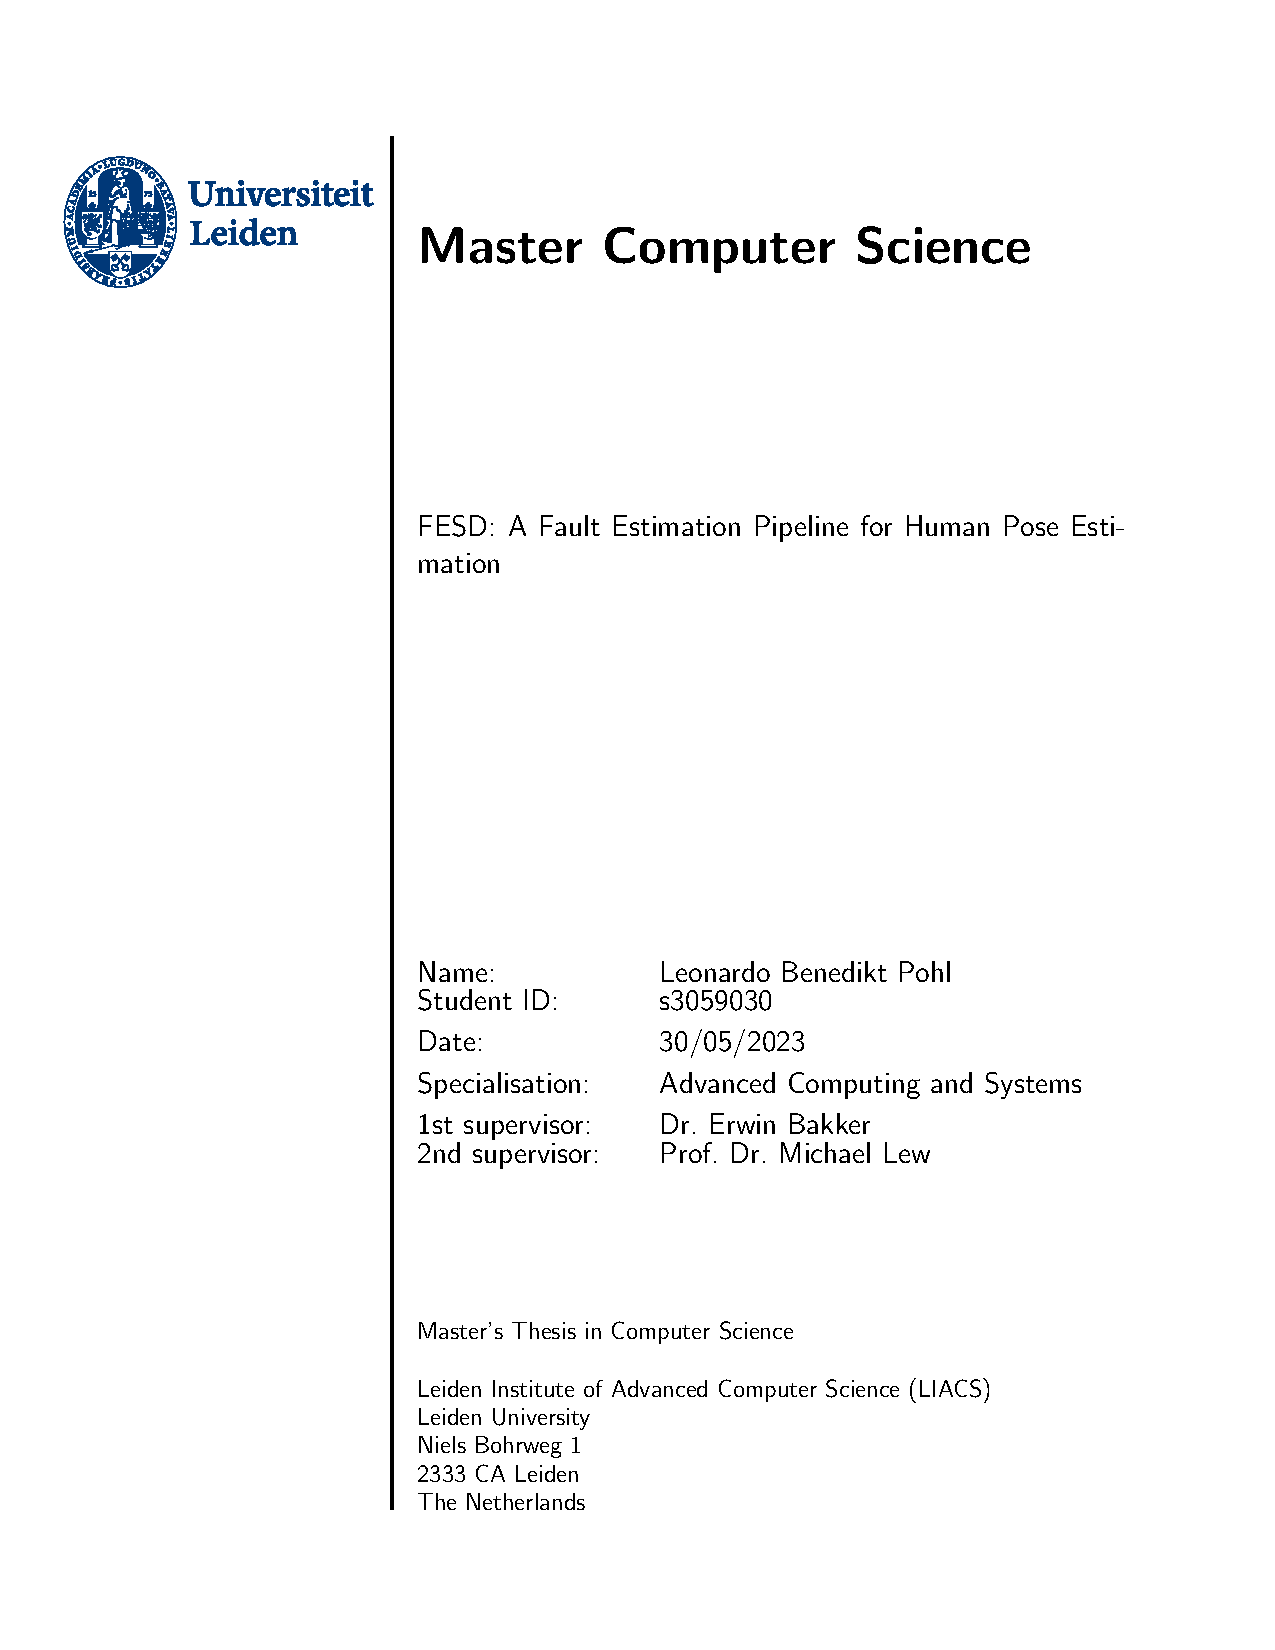
\includepdf[pages=1]{title_page.pdf}
\setlength{\voffset}{\originalVOffset}
\setlength{\hoffset}{\originalHOffset}

\cleardoublepage

\begin{abstract}  
  Human pose estimation(HPE), or skeleton detection, has been a topic of research for many years. With the advancement of hardware, it has become viable to apply HPE in real-time applications such as games. However, HPE is a difficult task that is prone to errors or faults, especially in complicated situations, such as cramped environments. These errors might cause human-computer interaction to be hampered.

  The goal of this thesis is to understand what causes the problems, and design exercises which deliberately cause common errors and to capture them within a dataset and label the entries accordingly. Finally, a preliminary method is developed to detect the errors or faults caused by HPE using the dataset.

  In the scope of this thesis, a method is developed that is capable of capturing and labelling multi-modal data, \textbf{F}ault \textbf{E}stimator for \textbf{S}keleton \textbf{D}etection \textbf{Data} processor (FESDData). I define four different problem sets with increasingly detailed areas, ranging from body-wise fault estimation to joint-wise fault estimation. Using the dataset, FESDDataset, that is recorded and labelled using FESDData, I developed one model for each problem set, which aims to detect if an error occurs at different levels, \textbf{F}ault \textbf{E}stimator for \textbf{S}keleton \textbf{D}etection \textbf{Model} (FESDModelv1 and FESDModelv2). While version one of the models uses custom feature extraction the second version uses transfer learning.

  In this thesis, I found common error sources that occur during HPE. Based on these I developed exercises which are captured in the FESDDataset using the dataset collection tool FESDData. The joints of the poses are then labelled based on the errors that occur. I abstracted the data to form four different problem sets, for each of which the two models, FESDModelv1 and FESDModelv2, are trained. The results of the model were at first promising, however, on further inspection proved to be overfitting since the data was insufficient and the model too complex. However, with further research and data FESDModelv1 and FESDModelv2 could be improved and, therefore, the way that HPE is evaluated could be changed by adding an extra level of verification.

\end{abstract}
